\documentclass[10pt,a4paper]{beamer}
\usepackage{amsmath, amssymb, mathtools}
\usepackage{amsthm}
\usepackage{fontspec}
\usepackage{xunicode}
\usepackage{fancyhdr}
\usepackage[french]{babel}
\usepackage{algorithm, algorithmic}
\usepackage{listings}
\usepackage{graphicx}
\usepackage{color}


\usetheme{Darmstadt}
\setbeamertemplate{navigation symbols}{}
\setbeamertemplate{blocks}[]
\usefonttheme[onlymath]{serif}

\institute{Sorbonne Université}
\title[Center text]{\textbf{Composition modulaire des polynômes à une variable}}
\subtitle{\small{Encadrant : M. Vincent NEIGER}}
\author{Serigne Fallou FALL \and Marie BONBOIRE}
\date{}


\begin{document}

\begin{frame}[plain]
    \titlepage
\end{frame}

\begin{frame}
    \tableofcontents
\end{frame}

\section{Introduction}
\begin{frame}{Introduction}
    Environnement :
    \begin{itemize}
        \item Corps d'étude : $\mathbb{Z}/p\mathbb{Z} := \{k | k\in\{0, ..., p-1\}\}$
        \item Implantation : Sagemath (Python), Flint (C) et NTL (C++)  
    \end{itemize}

    Notions primaires :
    \begin{itemize}
        \item addition, soustraction, division euclidienne
    \end{itemize}

    Notations  :
    \begin{itemize}
        \item $\tilde{O}$
    \end{itemize}
\end{frame}

%%%%%%%%%%%%%%%%%%%%%%%%%%%%%%%%%%%%%%%%
\section{Multiplication}
\begin{frame}{Multiplication}
    \begin{block}{Multiplication de polynômes}
        \textbf{Input :} $f,g \in \mathbb{Z}/p\mathbb{Z}[x]$ de degré au plus $n-1$ \\
        \textbf{Output :} $f \cdot g$
    \end{block}
    \rule{\linewidth}{0.2mm}\\[0.5cm]
    \textbf{Algorithme naïf}
    \[
    (f \cdot g)(x)=\sum_{i=0}^{2n-2} (\sum_{j+k=i}f_j \cdot g_k) \cdot x^i
    \]

    \begin{alertblock}{Complexité}
        L'algorithme naïf est en $O(n^2)$
    \end{alertblock}

\end{frame}

\begin{frame}
    \textbf{Algorithme de Karatsuba}
    \begin{align*}
        (f \cdot g)(x) &= \textcolor{blue}{F^{(0)} \cdot G^{(0)}}\\
            &+\left( \textcolor{green}{(F^{(0)}+F^{(1)}) \cdot (G^{(0)} + G^{(1)})} - \textcolor{blue}{F^{(0)} \cdot G^{(0)}} - \textcolor{red}{F^{(1)} \cdot G^{(1)}} \right)x^k\\
            &+ (\textcolor{red}{F^{(1)} \cdot G^{(1)}}) \cdot x^{2k} 
    \end{align*}

    \begin{alertblock}{Complexité}
        L'algorithme de Karatsuba est en $O(n^{log_2(3)})$
    \end{alertblock}
    \rule{\linewidth}{0.2mm}\\[0.5cm]

    
\end{frame}
    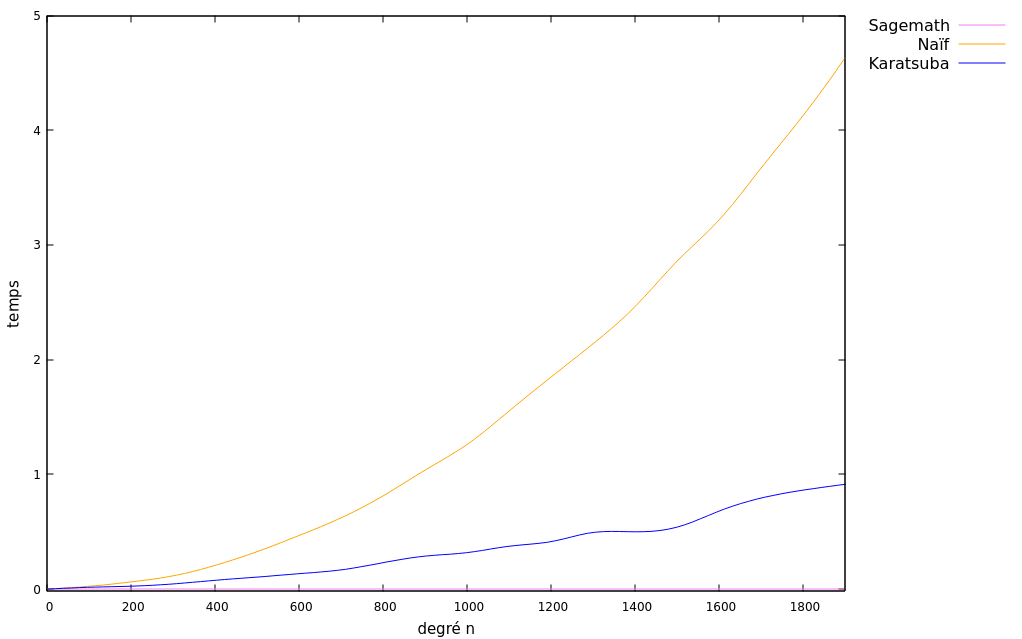
\includegraphics[width=0.5\linewidth]{multi.png}
\begin{frame}

\end{frame}

%%%%%%%%%%%%%%%%%%%%%%%%%%%%%%%%%%%%%%%%
\section{Composition modulaire}
\begin{frame}{Composition modulaire}
    \begin{block}{Composition modulaire}
        \textbf{Input :} $f \in \mathbb{Z}/p\mathbb{Z}[x]$ de degré n, $g \in \mathbb{Z}/p\mathbb{Z}[y]$ de degré $n$ \\ $a \in \mathbb{Z}/p\mathbb{Z}[x]$ de degré au plus $n-1$. \\
        \textbf{Output :} $g(a)\text{ mod }f$
    \end{block}
    \rule{\linewidth}{0.2mm}\\[0.5cm]
    
    \textbf{Algorithme naïf et Horner}
    \begin{align*} 
        g(a) \text{ mod }f &=(g_0+g_1\cdot a+g_2\cdot a^2+...+g_{n-1}\cdot a^{n-1}) \text{ mod } f \\
            &= ((...((g_{n-1}\cdot a)\text{ mod }f\ +\ g_{n-2})...)\cdot a)\text{ mod }f\ +\ g_0
    \end{align*}

    \begin{alertblock}{Complexité}
        L'algorithme naïf est en $\tilde{O}(n^3)$ tandis que l'algorithme d'Horner est en $\tilde{O}(n^2)$.
    \end{alertblock}
\end{frame}

\begin{frame}
    \textbf{Algorithme de Brent et Kung} 
    \begin{align*}
        g(x) &= g_0 + g_1y + ... + g_{\delta-1}y^{\delta-1} \\
            &+ y^\delta(g_\delta + g_{\delta+1}y + ... + g_{2\delta-1}y^{\delta-1}) \\
                                          &+ y^{2\delta}(g_{2\delta} + g_{2\delta+1}y + ... + g_{3\delta-1}y^{\delta-1}) \\
                                          &+ ... \\
                                          &+ y^{\delta(\delta-1)}(g_{\delta(\delta-1)} + g_{\delta(\delta-1)+1}y + ... + g_{\delta^2-1}y^{\delta-1}) 
    \end{align*}
    \[
    g(y) = 
    \begin{pmatrix}
        1 \\
        y^\delta \\
        \vdots \\
        (y^\delta)^{\delta-1} 
    \end{pmatrix}^t
    \begin{pmatrix}
        g_0 & g_1 & ... & g_{\delta-1} \\
        g_{\delta} & g_{\delta+1} & ... & g_{2\delta-1} \\
        \vdots & ... & \vdots \\
        g_{\delta(\delta-1)} & g_{\delta(\delta-1)+1} & ... & g_{\delta^2-1}
    \end{pmatrix}
    \begin{pmatrix}
        1 \\
        y \\
        \vdots \\
        y^{\delta-1}
    \end{pmatrix}
    \]
    
    \[
        \begin{pmatrix}
            1 \\
            a \text{ mod }f\\
            \vdots \\
            a^{\delta-1} \text{ mod }f
        \end{pmatrix}
        =
        \begin{pmatrix}
            1 & 0 & ... & 0 \\
            a_{1,0} & a_{1,1} & ... & a_{1,n-1} \\
            \vdots & \vdots & ... & \vdots \\
            a_{\delta-1,0} & a_{\delta-1,1} & ... & a_{\delta-1,n-1}
        \end{pmatrix}
        \begin{pmatrix}
            1 \\
            x \\
            \vdots \\
            x^{\delta-1}
        \end{pmatrix}
    \]
\end{frame}

\begin{frame}
    \[
    \begin{pmatrix}
        1 \\
        y^\delta \\
        \vdots \\
        (y^\delta)^{\delta-1} 
    \end{pmatrix}^t
    \begin{pmatrix}
        g_0 & ... & g_{\delta-1} \\
        g_1 & ... & g_{2\delta-1} \\
        \vdots & ... & \vdots \\
        g_{\delta(\delta-1)} & ... & g_{\delta^2-1}
    \end{pmatrix}
    \begin{pmatrix}
        1 &  ... & 0 \\
        a_{1,0} & ... & a_{1,n-1} \\
        \vdots &  ... & \vdots \\
        a_{\delta-1,0} & ... & a_{\delta-1,n-1}
    \end{pmatrix}
    \begin{pmatrix}
        1 \\
        x \\
        \vdots \\
        x^{\delta-1}
    \end{pmatrix}
    \]
    \rule{\linewidth}{0.2mm}\\[0.5cm]
    \[
    \begin{pmatrix}
        B_0 \\
        B_1 \\
        \vdots \\
        B_d
    \end{pmatrix}
    =
    \begin{pmatrix}
        g_0 & ... & g_{d-1} \\
        g_1 & ... & g_{2d-1} \\
        \vdots & ... & \vdots \\
        g_{d(d-1)} & ... & g_{d^2-1}
    \end{pmatrix}
    \begin{pmatrix}
        1 & 0 & ... & 0 \\
        a_{1,0} & a_{1,1} & ... & a_{1,n-1} \\
        \vdots & \vdots & ... & \vdots \\
        a_{d,0} & a_{d,1} & ... & a_{d,n-1}
    \end{pmatrix} 
    \]
    \begin{itemize} 
        \item Retourne horner(B, $a^{\delta}$, $f$)
    \end{itemize}
    \begin{alertblock}{Complexité}
        L'algorithme de Brent et Kung est en $O((1+n/d)d^{\omega_2/2})$
    \end{alertblock}
\end{frame}

\begin{frame}
    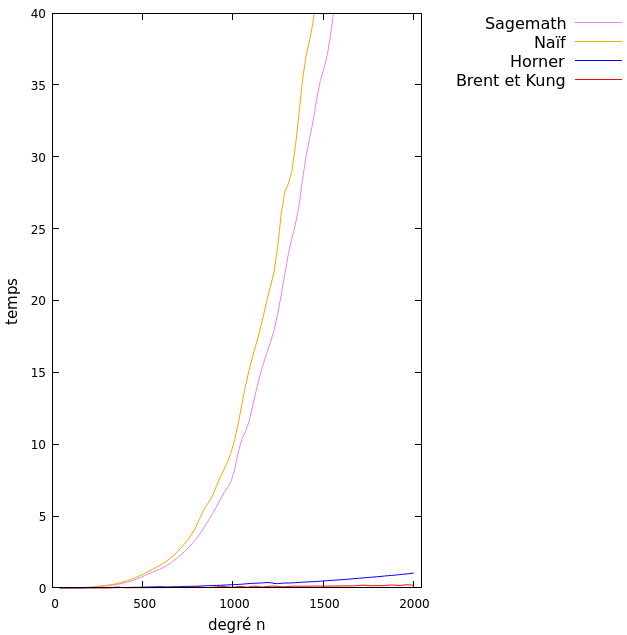
\includegraphics[width=1\linewidth]{comp.png}
\end{frame}

\begin{frame}
    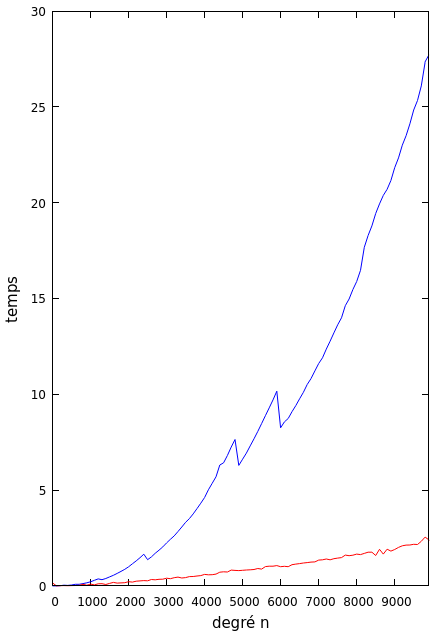
\includegraphics[width=1\linewidth]{comp_2.png}
\end{frame}

%%%%%%%%%%%%%%%%%%%%%%%%%%%%%%%%%%%%%%%%%%ù
\section{Algorithme de Nüsken et Ziegler}
\begin{frame}{Algorithme de Nüsken et Ziegler}
    \begin{block}{Nusken et Ziegler}
        \textbf{Input :} $f \in \mathbb{Z}/p\mathbb{Z}[X]$ de degré $n$, $g \in \mathbb{Z}/p\mathbb{Z}[x,y]$ de degré $n$ $a \in \mathbb{Z}/p\mathbb{Z}[X]$ de degré au plus $n-1$. \\
        \textbf{Output :} g(a) mod f
    \end{block}

    \[
    g(x,y) = \sum_{i,j<\delta}g_{i+\delta j}(x)y^{i+\delta j} = \sum_{j<\delta} \left( \sum_{i<\delta} g_{i+\delta j}(x)y^i \right) y^{\delta j}     
    \]

    \begin{itemize}
        \item Calcul simultané des $R_j = g_{i+\delta j}(x)a^i \%f $
            \[
            \begin{pmatrix}
                R_0 \\
                R_1 \\
                \vdots \\
                R_{\delta-1}
            \end{pmatrix}
            =
            \begin{pmatrix}
                g_0(x)&g_1(x)&...&g_{\delta -1}(x) \\
                g_{\delta}(x)&g_{1+\delta}(x)&...&g_{2\delta-1}(x) \\
                \vdots&\vdots&...&\vdots \\
                g_{(\delta-1)\delta}(x)&g_{(\delta-1)\delta+1}(x)&...&g_{\delta^2-1}(x)
            \end{pmatrix}
            \begin{pmatrix}
                1 \\
                a \\
                a^2 \%f \\
                ... \\
                a^{\delta-1} \%f
            \end{pmatrix}
            \]
        \item Pour $j\in{0,...,\delta-1}$, $a_j=a^{\delta j}\% f$
        \item Retourne $\sum_{j<\delta}(R_ja_j \% f)$
    \end{itemize}

    
\end{frame}

\begin{frame}
    \begin{alertblock}{Complexité}
        L'algorithme de Nusken et Ziegler est en $O(d_yM(d_x) + d_yM(n))$
    \end{alertblock}
\end{frame}

\section{Conclusion}

\end{document}
